\section{Operations Research workflow}

\begin{figure}[H]
    \centering
    
\includegraphics[width=1\linewidth]{images/study.png}
\end{figure}
The fundamental stages involved in the examination of an Operations Research problem are as follows:
\begin{enumerate}
    \item Problem definition: the initial step is to precisely articulate and understand the problem at hand.
    \item Model construction: subsequently, a mathematical or computational model is constructed to encapsulate the problem's complexity.
    \item Algorithm selection or development: to solve the model, an appropriate algorithm is chosen or developed, tailored to the specifics of the problem.
    \item Implementation: the selected algorithm is either implemented or utilized within an existing software or program.
\end{enumerate}
Upon completing this process, the results are thoroughly scrutinized, and feedback is integrated.

The resultant model, forged through this procedure, serves as a simplified representation of the real-world problem. 
To define it effectively, one must discern the fundamental components of the problem and delineate the principal relationships among them.
\begin{example}
    A company produces three types of electronic devices: $D_1,D_2,D_3$, which go through three main phases of the production process: assembly, refinement, and quality control.
    The time required for each phase and product is as follows:
    \begin{table}[H]
        \centering
        \begin{tabular}{c|ccc|}
        \cline{2-4}
        \textbf{}                             & \textbf{$D_1$} & \textbf{$D_2$} & $D_3$ \\ \hline
        \multicolumn{1}{|c|}{Assembly}        & 80             & 70             & 120   \\
        \multicolumn{1}{|c|}{Refinement}      & 70             & 90             & 20    \\
        \multicolumn{1}{|c|}{Quality control} & 40             & 30             & 20    \\ \hline
        \end{tabular}
    \end{table}
    The available resources within the planning horizon, in minutes, are:
    \begin{table}[H]
        \centering
        \begin{tabular}{|c|c|c|}
        \hline
        \textbf{Assembly} & \textbf{Refinement} & \textbf{Quality control} \\ \hline
        30 000            & 25 000              & 18 000                   \\ \hline
        \end{tabular}
    \end{table}
    The unary product for each product is: 
    \begin{table}[H]
        \centering
        \begin{tabular}{|c|c|c|}
        \hline
        $D_1$          & $D_2$          & $D_3$ \\ \hline
        1600           & 1000           & 2000  \\ \hline
        \end{tabular}
    \end{table}
    The main assumption is that the company can sell whatever it produces.

    The mathematical model that describes this problem is as follows:
    \begin{itemize}
        \item Decision variables: $x_j$ represents the number of devices $D_j$ produced for $j=1,2,3$.
        \item Objective function: we need to maximize earnings, so we have: 
            \[\max{\left[1.6x_1+1x_2+2x_3\right]}\]
        \item Constraints: the constraints are based on the production limits of each phase:
            \[80x_1+70x_2+120x_3 \leq 30000\]
            \[70x_1+90x_2+20x_3 \leq 25000\]
            \[40x_1+30x_2+20x_3 \leq 18000\]
        \item Variable type: the variables must be non-negative values, so we have $x_1,x_2,x_3 \geq 0$.
    \end{itemize}
\end{example}
\begin{example}
    An insurance company must decide which investments to select out of a given set of possible assets.
    Here is the information about the investments:
    \begin{table}[H]
        \centering
        \begin{tabular}{|c|ccc|}
        \hline
        \textbf{Investments} & \textbf{Area} & \textbf{Capital ($c_j$)} & \textbf{Return ($r_j$)} \\ \hline
        A (automotive)       & Germany       & $150 000$                & $11\%$                  \\
        B (automotive)       & Italy         & $150 000$                & $9\%$                   \\
        C (ICT)              & USA           & $60 000$                 & $13\%$                  \\
        D (ICT)              & Italy         & $100 000$                & $10\%$                  \\
        E (real estate)      & Italy         & $125 000$                & $8\%$                   \\
        F (real estate)      & France        & $100 000$                & $7\%$                   \\
        G (treasury bonds)   & Italy         & $50 000$                 & $3\%$                   \\
        H (treasury bonds)   & UK            & $80 000$                 & $5\%$                   \\ \hline
        \end{tabular}
    \end{table}
    The available capital is 600,000 Euro.
    The company is required to make at most five different investments, with a maximum of three investments in Italy and a maximum of three abroad.

    The mathematical model for this problem is as follows:
    \begin{itemize}
        \item Decision variables: binary variables $x_j$ that indicate whether the $j$-th investment is selected ($x_j=1$) or not ($x_j=0$), for $j=0,\dots, 8$.          
        \item Objective function: we need to maximize the expected return, so the objective function is:
            \[\max{\left[\sum_{j=1}^8{c_jr_jx_j}\right]}\]
        \item Constraints: there is a constraint on the total capital invested, ensuring it doesn't exceed the available capital:
            \[\sum_{j=1}^8{c_jx_j} \leq 800\]
            There is a constraint on the maximum number of investments, which should be at most five:
            \[\sum_{j=1}^8{x_j} \leq 5\]
            Constraints on the maximum number of investments in Italy (at most three) and abroad (at most three):
            \[x_2+x_4+x_5+x_7 \leq 3\]
            \[x_1+x_3+x_6+x_8 \leq 3\]
        \item Variable type: the variables are binary integer defined as $x_j \in \{0,1\} \:\: 1 \leq j \leq 8$. 
    \end{itemize}
    The variant of the problem introduces an additional constraint. 
    If any of the ICT investments (C or D) is selected, then at least one of the treasury bonds (G or H) must be selected. 
    The constraint is as follows:
    \[\dfrac{x_3+x_4}{2} \leq x_7+x_8\]
    This constraint ensures that if both ICT investments are selected, at least one treasury bond must also be selected (not both).
\end{example}
\begin{example}
    There are three oil pits located at points $A=(0,0)$, $B=(300,0)$, and $C=(240,300)$, and the goal is to connect them to a refinery with pipelines.
    \begin{figure}[H]
        \centering
        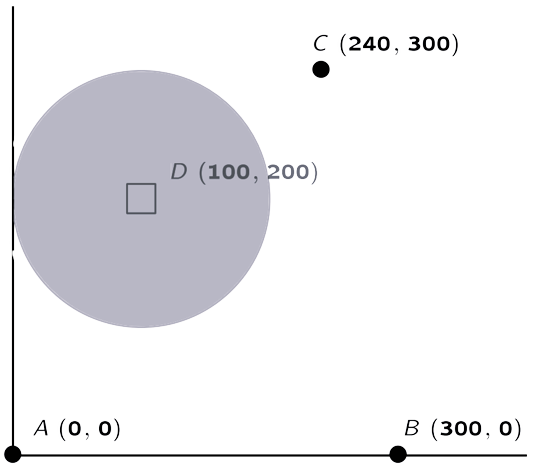
\includegraphics[width=0.4\linewidth]{images/example3.png}
    \end{figure}
    The cost of the pipelines is proportional to the square of their length.
    The refinery must be at least 100 km away from point $D=(100,200)$.
    The objective is to find the location for the refinery that minimizes the total pipeline cost.

    The mathematical model for this problem can be defined as follows:
    \begin{itemize}
        \item Decision variables: the coordinates of the refinery, denoted as $x_1,x_2$. 
        \item Objective function: we need to minimize the total pipeline cost, which is the sum of the squared distances between the oil pits and the refinery:
        \begin{align*}
            \min{z} &=\left[ (x_1-0)^2+(x_2-0)^2 \right] \\
                    &+ \left[ (x_1-300)^2+(x_2-0)^2 \right] \\
                    &+ \left[ (x_1-240)^2+(x_2-300)^2 \right] 
        \end{align*}
        \item Constraints: there is a constraint that ensures the refinery is at least 100 km away from point $D=(100,200)$. 
            The constraint can be represented as:
            \[\sqrt{{\left( x_1-100 \right)}^2+{\left( x_2-100 \right)}^2} \geq 100\]
        \item Variable type: $x_1,x_2 \in \mathbb{R}$
    \end{itemize}
\end{example}